%%%%%%%%%%%%%%%%%%%%%%%%%%%%%%%%%%%%%%%%%%%%%%%%%%%%%%%%%%%%
%%  Class 35, NE 155
%%

\documentclass[xcolor=x11names,compress]{beamer}

\definecolor{CoolBlack}{rgb}{0.0, 0.18, 0.39}
%% General document %%%%%%%%%%%%%%%%%%%%%%%%%%%%%%%%%%
\usepackage{graphicx}
\usepackage{tikz}
\usetikzlibrary{decorations.fractals}
\usepackage{hyperref}
%%%%%%%%%%%%%%%%%%%%%%%%%%%%%%%%%%%%%%%%%%%%%%%%%%%%%%

%% Beamer Layout %%%%%%%%%%%%%%%%%%%%%%%%%%%%%%%%%%
\useoutertheme[subsection=false,shadow]{miniframes}
\useinnertheme{default}
\usefonttheme{serif}
\usepackage{palatino}
\usepackage{tabu}
\usepackage[normalem]{ulem}
% Links
\usepackage{hyperref}
\definecolor{links}{HTML}{003262}
\hypersetup{colorlinks,linkcolor=,urlcolor=links}

% addition of color
\usepackage{xcolor}
\definecolor{CoolBlack}{rgb}{0.0, 0.18, 0.39}
\definecolor{byellow}{rgb}{0.55037, 0.38821, 0.06142}
\definecolor{dgreen}{rgb}{0.,0.6,0.}
\definecolor{RawSienna}{cmyk}{0,0.72,1,0.45}
\definecolor{forestgreen(web)}{rgb}{0.13, 0.55, 0.13}
\definecolor{cardinal}{rgb}{0.77, 0.12, 0.23}

\setbeamerfont{title like}{shape=\scshape}
\setbeamerfont{frametitle}{shape=\scshape}

\setbeamercolor*{lower separation line head}{bg=CoolBlack}
\setbeamercolor*{normal text}{fg=black,bg=white}
\setbeamercolor*{alerted text}{fg=dgreen} % just testing; I think this looks better
\setbeamercolor*{example text}{fg=black}
\setbeamercolor*{structure}{fg=black}

\setbeamercolor*{palette tertiary}{fg=black,bg=black!10}
\setbeamercolor*{palette quaternary}{fg=black,bg=black!10}

% Margins
\usepackage{changepage}

\mode<presentation>
{
  \definecolor{berkeleyblue}{HTML}{003262}
  \definecolor{berkeleygold}{HTML}{FDB515}
  \usetheme{Boadilla}      % or try Darmstadt, Madrid, Warsaw, Boadilla...
  %\usecolortheme{dove} % or try albatross, beaver, crane, ...
  \setbeamercolor{structure}{fg=berkeleyblue,bg=berkeleygold}
  \setbeamercolor{palette primary}{bg=berkeleyblue,fg=white} % changed this
  \setbeamercolor{palette secondary}{fg=berkeleyblue,bg=berkeleygold} % changed this
  \setbeamercolor{palette tertiary}{bg=berkeleyblue,fg=white} % changed this
  \usefonttheme{structurebold}  % or try serif, structurebold, ...
  \useinnertheme{circles}
  \setbeamertemplate{navigation symbols}{}
  \setbeamertemplate{caption}[numbered]
  \usebackgroundtemplate{}
}
%---

\renewcommand{\(}{\begin{columns}}
\renewcommand{\)}{\end{columns}}
\newcommand{\<}[1]{\begin{column}{#1}}
\renewcommand{\>}{\end{column}}

% adding slide numbers
\addtobeamertemplate{navigation symbols}{}{%
    \usebeamerfont{footline}%
    \usebeamercolor[fg]{footline}%
    \hspace{1em}%
    \insertframenumber/\inserttotalframenumber
}

% equation stuff
\newcommand{\Macro}{\ensuremath{\Sigma}}
\newcommand{\Sn}{\ensuremath{S_N} }
\newcommand{\vOmega}{\ensuremath{\hat{\Omega}}}
\usepackage{mathrsfs}
\usepackage[mathcal]{euscript}
\usepackage{amssymb}
\usepackage{amsthm}
\usepackage{epsfig}
\usepackage{amsmath}
%%%%%%%%%%%%%%%%%%%%%%%%%%%%%%%%%%%%%%%%%%%%%%%%%%
% title stuff for footer
\title{NE 155}
\author{R.\ N.\ Slaybaugh \\
(well, Katy Huff actually)}
\date{April 22, 2015}

\begin{document}

%%%%%%%%%%%%%%%%%%%%%%%%%%%%%%%%%%%%%%%%%%%%%%%%%%%%%%
%%%%%%%%%%%%%%%%%%%%%%%%%%%%%%%%%%%%%%%%%%%%%%%%%%%%%%
\begin{frame}
\title{NE 155\\Introduction to Numerical Simulations in Radiation Transport}
\subtitle{Lecture 35: Estimators and Tallies}
\titlepage
\end{frame}


%%%%%%%%%%%%%%%%%%%%%%%%%%%%%%%%%%%%%%%%%%%%%%%%%%%%%%
%%%%%%%%%%%%%%%%%%%%%%%%%%%%%%%%%%%%%%%%%%%%%%%%%%%%%%
\begin{frame}{Outline}

    \begin{enumerate}
    \item Tally \& Estimator Basics
    \item Surface Current Tally
    \item Flux Tallies and Estimators
    \item Energy Deposition Tallies and Estimators
    \item Pulse Height Tally
    \item Detector Tallies
    \end{enumerate}

\vspace*{1em}
Notes derived from Jasmina Vujic and Paul Wilson
\end{frame}



%%%%%%%%%%%%%%%%%%%%%%%%%%%%%%%%%%%%%%%%%%%%%%%%%%%%%%
%%%%%%%%%%%%%%%%%%%%%%%%%%%%%%%%%%%%%%%%%%%%%%%%%%%%%%
\begin{frame}{Learning Objectives}

    \begin{enumerate}
    \item Understand relationship between tallies
and estimators
    \item Explain derivation of volume and
surface track length estimators
    \item Demonstrate difference between track
length energy deposition estimator and
pulse height tally
    \item Understand next-event estimator and
its application to point detectors
    \end{enumerate}

NOTE: The rest of this is a copy of the xport talk and isn't actually this talk!

\end{frame}


%%%%%%%%%%%%%%%%%%%%%%%%%%%%%%%%%%%%%%%%%%%%%%%%%%%%%%
%%%%%%%%%%%%%%%%%%%%%%%%%%%%%%%%%%%%%%%%%%%%%%%%%%%%%%
\begin{frame}{Monte Carlo for Transport}

  	\begin{figure}
  	\begin{center}
  		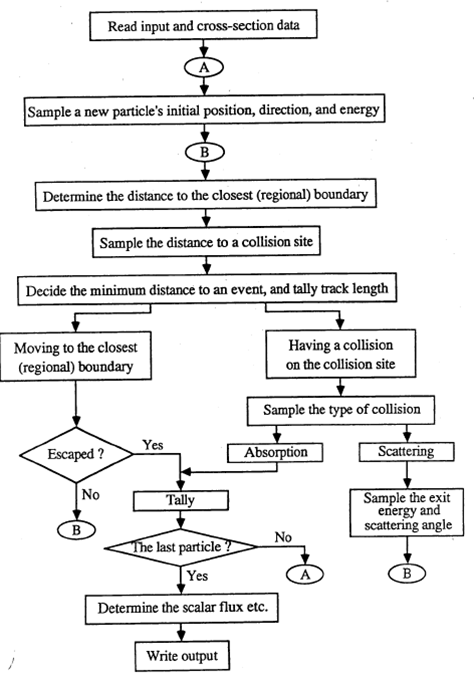
\includegraphics[height=3in,clip]{MC-algorithm}
	\end{center}
  	\end{figure}
  	% we've covered some of the basics that surround this algorithm,
  	% today we'll start covering some of the nuts and bolts
  	% Next time we'll cover tallies.
  	
\end{frame}


%%%%%%%%%%%%%%%%%%%%%%%%%%%%%%%%%%%%%%%%%%%%%%%%%%%%%%
%%%%%%%%%%%%%%%%%%%%%%%%%%%%%%%%%%%%%%%%%%%%%%%%%%%%%%
\begin{frame}{Possible Futures for a Particle}

After we've gotten to \alert{Circle B}, we have a neutral particle:
\begin{itemize}
  \item At point $(x_p , y_p , z_p)$
  \item Moving in direction $(u, v, w)$
  \item With energy $E$
\end{itemize}
What are possible next events?
\pause
  	\begin{figure}
  	\begin{center}
  		\includegraphics<2>[height=1.25in,clip]{collision}
  		\includegraphics<3>[height=1.25in,clip]{boundary-xing}
  		\caption{\only<2>{Collision}\only<3>{Surface Crossing}}
	\end{center}
  	\end{figure}

\end{frame}


%%%%%%%%%%%%%%%%%%%%%%%%%%%%%%%%%%%%%%%%%%%%%%%%%%%%%%
%%%%%%%%%%%%%%%%%%%%%%%%%%%%%%%%%%%%%%%%%%%%%%%%%%%%%%
\begin{frame}{Sampling Distance to Collision}

Collisions are probabilistic
\begin{itemize}
  \item Note that $\Sigma_t$, the total macroscopic cross section, will be a function of space if we have multiple materials
  \item Along a particular path, the \textit{probability of a collision at distance $s$} from the start:
    \begin{align*}
    p_c(s) &= \Sigma_t(s) e^{-\Sigma_t(s) s} ds \\
    P_c(n) &= \int_0^s \Sigma_t(s) e^{-\Sigma_t(s) s'}ds' = -e^{-\Sigma_t(s) s'} |_0^s = 1 - e^{-\Sigma_t(s) s}
  \end{align*}
  %\item This is the probability of interaction per unit distance $\times$ probability of traveling $s$ without interacting
%  \vspace*{0.5 em}
%  \pause
  \item The cross section, $\Sigma_t(s)$, is piecewise constant, \underline{but changing}
%  \item Integrating along path: CDF is piecewise
\end{itemize}
%  	\begin{figure}
%  	\begin{center}
%  		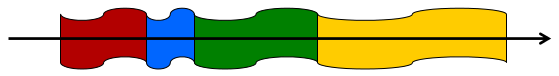
\includegraphics[height=.33in,clip]{xsec-cdf}
%	\end{center}
%  	\end{figure}

\end{frame}


%%%%%%%%%%%%%%%%%%%%%%%%%%%%%%%%%%%%%%%%%%%%%%%%%%%%%%
%%%%%%%%%%%%%%%%%%%%%%%%%%%%%%%%%%%%%%%%%%%%%%%%%%%%%%
\begin{frame}{Sampling Distance to Collision}

\begin{itemize}
  \item Variable transformation: measure distance in units of \textit{mean free path}:
  \[n = \Sigma_t(s)s\:,\quad dn = \Sigma_t(s)ds\]
  \item We'll start with the PDF and integrate to get the CDF
 \begin{align*}
    p_c(n)dn &= e^{-n} dn\\
    P_c(n) &= \int_0^n e^{-n'}dn' = -e^{-n'} |_0^n = 1 - e^{-n}
  \end{align*}
  \item Importantly, this is now \underline{independent of the material}
\end{itemize} 

\end{frame}


%%%%%%%%%%%%%%%%%%%%%%%%%%%%%%%%%%%%%%%%%%%%%%%%%%%%%%
%%%%%%%%%%%%%%%%%%%%%%%%%%%%%%%%%%%%%%%%%%%%%%%%%%%%%%
\begin{frame}{Sampling Distance to Collision}

Randomly sample to determine number of mean free paths until next collision, $n_c$

\begin{itemize}
  \item $g(n_c) dn_c = e^{-n_c} dn_c$ 
  \vspace{.5em}
  \item $G(n_c) dn_c = 1 - e^{-n_c}$ 
  \vspace{.5em}
  \item Directly invert to get: $\boxed{n_c = - \ln(1 - \xi)}$ \\
   \hspace*{1.5em} (note $1-\xi$ is equivalent to $\xi$)
  \vspace{.5em}
  \item In the absence of material boundaries ($\Sigma \neq f(s)$), the distance to a collision, $s_c$, is
  \[s_c = \frac{n_c}{\Sigma_t}\]
\end{itemize}

\end{frame}


%%%%%%%%%%%%%%%%%%%%%%%%%%%%%%%%%%%%%%%%%%%%%%%%%%%%%%
%%%%%%%%%%%%%%%%%%%%%%%%%%%%%%%%%%%%%%%%%%%%%%%%%%%%%%
\begin{frame}{Calculating Distance to Boundary}

\begin{itemize}
  \item Usually have \textit{more than one material}
  \vspace*{1 em}
  \item Distance to boundary is deterministic
  \vspace*{1 em}
  \item Algebra to determine distance between point and surface, $s_b$
  \vspace*{1 em}
  \item Convert it to units of mean free path for the current cell's material, 
  \[n_b = s_b \Sigma_t\] 
\end{itemize}

\end{frame}


%%%%%%%%%%%%%%%%%%%%%%%%%%%%%%%%%%%%%%%%%%%%%%%%%%%%%%
%%%%%%%%%%%%%%%%%%%%%%%%%%%%%%%%%%%%%%%%%%%%%%%%%%%%%%
\begin{frame}{Geometry Representations}

\begin{itemize}
  \item Combinatorial Surfaces
  \begin{itemize}
    \item Define surfaces
    \item Boolean operations combine surfaces to create cells
  \end{itemize}
  \vspace*{1 em}
  \item Combinatorial Solids
  \begin{itemize}
    \item Choose solid objects
    \item Boolean operations combine objects to create regions
  \end{itemize}
  \vspace*{1 em}
  \item B-Rep (Vertex-Edge)
  \begin{itemize}
    \item Each object is a single set of vertices and edges connecting them
  \end{itemize}
\end{itemize}
\vspace*{1 em}
We're skipping how to find $n_b$, just know that we can find it

\end{frame}


%%%%%%%%%%%%%%%%%%%%%%%%%%%%%%%%%%%%%%%%%%%%%%%%%%%%%%
%%%%%%%%%%%%%%%%%%%%%%%%%%%%%%%%%%%%%%%%%%%%%%%%%%%%%%
\begin{frame}{Option A: Collision}

  \underline{$n_b > n_c$}:
  \begin{itemize}
    \item Boundary is further away than collision
    \item \alert{Collision occurs}
  \end{itemize}
    \vspace*{0.5 em}
  \pause

\begin{itemize}
  \item Using physics models and/or cross-sections
  \begin{itemize}
    \item Sample target nuclide
    \item Sample reaction type
    \item Sample new direction 
    \item Sample new energy 
    \item Sample exiting particles 
  \end{itemize}
  \item Some of these may depend on each other
  \vspace*{0.5 em}
  \pause
  \item Repeat
  \begin{itemize}
    \item Sample new $n_c$ following collision
    \item Calculate new $n_b$ in new direction
  \end{itemize}
\end{itemize}


\end{frame}

%%%%%%%%%%%%%%%%%%%%%%%%%%%%%%%%%%%%%%%%%%%%%%%%%%%%%%
%%%%%%%%%%%%%%%%%%%%%%%%%%%%%%%%%%%%%%%%%%%%%%%%%%%%%%
\begin{frame}{Option B: Cell Boundary}

  \underline{$n_b < n_c$}:
  \begin{itemize}
    \item Boundary is closer than collision
    \item \alert{Boundary crossing occurs}
  \end{itemize}
    \vspace*{0.5 em}
  \pause

  \begin{itemize}
  \item Move particle along ray
  \begin{itemize}
    \item Update $n_c = n_c - n_b$
  \end{itemize}
  \item \textbf{DO NOT SAMPLE} for new $n_c$
  \vspace*{1 em}
  \pause
  \item Calculate new $n_b$ in new cell
  \begin{itemize}
    \item New set of boundaries
    \item New value of $\Sigma_t$
  \end{itemize}
\end{itemize}

\end{frame}


%%%%%%%%%%%%%%%%%%%%%%%%%%%%%%%%%%%%%%%%%%%%%%%%%%%%%%
%%%%%%%%%%%%%%%%%%%%%%%%%%%%%%%%%%%%%%%%%%%%%%%%%%%%%%
\begin{frame}{So You Had a Collision?}

\begin{itemize}
  \item Sample \textbf{target nuclide} for a mixture with $J$ nuclides
    \[\Sigma_t = \sum_{j=1}^J N_j \sigma_{t,j}\]
  \item \textit{Discrete PDF} to determine which nuclide is hit
    \[p_i = \frac{\Sigma_{t,j}}{\Sigma_t}\]
  \pause
  \item Sample \textbf{reaction type} for an nuclide with R types of reactions
     \[\Sigma_{t,j} = \sum_{x=1}^R \Sigma_{x,j}\]
  \item \textit{Discrete PDF} to determine which reaction occurs
    \[p_x = \frac{\Sigma_{x,j}}{\Sigma_{t,j}}\]
\end{itemize}

\end{frame}


%%%%%%%%%%%%%%%%%%%%%%%%%%%%%%%%%%%%%%%%%%%%%%%%%%%%%%
%%%%%%%%%%%%%%%%%%%%%%%%%%%%%%%%%%%%%%%%%%%%%%%%%%%%%%
\begin{frame}{Outcome of Reaction}

\begin{itemize}
    \item Particle maybe absorbed
\vspace*{1em}
    \item Particle may continue its history in a \textit{different direction} and with a \textit{different energy}
\vspace*{1em}
    \item Energy-angle distributions are tabulated in different formats
    \begin{itemize}
      \item Scattering laws have analytic forms with parameters in data tables\\
      (Direct inversion or rejection sampling)
      \item Tabulated data that describes a piecewise analytic interpolation\\
      (Hybrid sampling; we skipped this)
    \end{itemize}
\end{itemize}

\end{frame}


%%%%%%%%%%%%%%%%%%%%%%%%%%%%%%%%%%%%%%%%%%%%%%%%%%%%%%
%%%%%%%%%%%%%%%%%%%%%%%%%%%%%%%%%%%%%%%%%%%%%%%%%%%%%%
\begin{frame}{Using a Scattering Angle}

Scattering angles are defined relative to the original direction (considered as the z-axis)

\begin{itemize}
    \item Polar angle, $\phi$, determined by sampling from data
\vspace*{0.5em}
    \item Azimuthal angle, $\theta$, determined by sampling isotropically
    \vspace*{0.5em}
   % \item Consider old/original direction as the z-axis in a different coordinate system
    \item The new direction is $\bigl(\sin(\phi) \cos(\theta), \sin(\phi) \sin(\theta), \cos(\theta)\bigr)$ \[= \bigl(\sqrt{1 - \mu^2} \cos(\theta),  \sqrt{1 - \mu^2} \sin(\theta), \mu \bigr)\]
\end{itemize}

  	\begin{figure}
  	\begin{center}
  		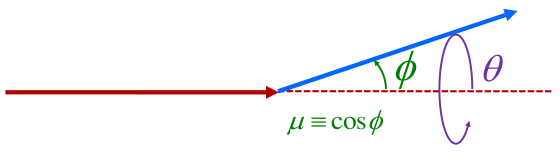
\includegraphics[height=1in,clip]{scattering-angle-2}
	\end{center}
  	\end{figure}

\end{frame}


%%%%%%%%%%%%%%%%%%%%%%%%%%%%%%%%%%%%%%%%%%%%%%%%%%%%%%
%%%%%%%%%%%%%%%%%%%%%%%%%%%%%%%%%%%%%%%%%%%%%%%%%%%%%%
\begin{frame}{Summary}

We've developed a general sense of using MC for neutron transport
\begin{itemize}
    \item Basic Algorithm
    \pause
    \vspace*{0.5 em}
    \item We can determine if particles have collisions or cross boundaries
    \item \textit{After a collisions} we need to determine many things associated with the collisions (target, reaction, direction, energy)
    \item Repeat analysis for collisions/crossing until particle \textbf{terminates}
    \pause
    \vspace*{0.5 em}
    \item Next time: tallying results
\end{itemize}


\end{frame}



\end{document}
